\section[Адаптивная сеть на основе системы нечеткого вывода]{%
  АДАПТИВНАЯ СЕТЬ НА ОСНОВЕ СИСТЕМЫ \\
  НЕЧЕТКОГО ВЫВОДА
}

Для осуществления нечеткого логического вывода
гибридные нейроны объединяются в сеть, как показано на рисунке~\ref{fig:anfis}.
В зарубежной литературе приведенная архитектура носит название ANFIS
(от англ. Adaptive Neuro-Fuzzy Inference System).

\begin{figure}[h!]
  \centering
  \fcolorbox{gray}{white}{
    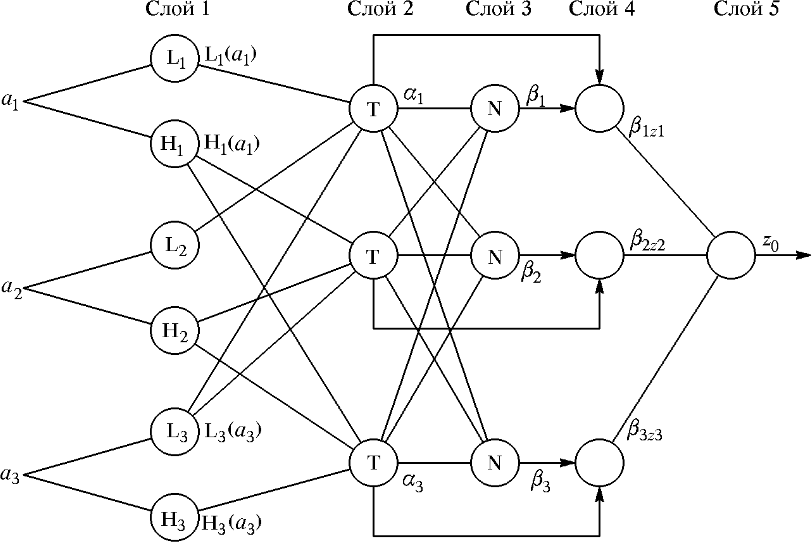
\includegraphics[width=120mm]{fig/anfis}
  }
  \caption{Структура гибридной нейронной сети \\ (архитектура ANFIS)}
  \label{fig:anfis}
\end{figure}

Рассмотрим структуру данной сети, принимая во внимание, что она соответствует
следующему набору правил: \par
\( \text{П}_1 \): если
\( x_1 \) есть \( L_1 \) и
\( x_2 \) есть \( L_2 \) и
\( x_3 \) есть \( L_3 \),
то \( y \) есть \( H \), \par
\( \text{П}_2 \): если
\( x_1 \) есть \( H_1 \) и
\( x_2 \) есть \( H_2 \) и
\( x_3 \) есть \( L_3 \),
то \( y \) есть \( M \), \par
\( \text{П}_3 \): если
\( x_1 \) есть \( H_1 \) и
\( x_2 \) есть \( H_2 \) и
\( x_3 \) есть \( H_3 \),
то \( y \) есть \( S \).

\pagebreak

Выходы узлов первого слоя представляют собой значения функции
принадлежности при заданных значениях входов.
Выходы второго слоя соответствуют значениям истинности условной части
каждого правила вывода, вычисляемые по формулам:
\[
  \begin{aligned}
    \alpha_1 &= L_1(a_1) \cap L_2(a_2) \cap L_3(a_3), \\
    \alpha_2 &= H_1(a_1) \cap H_2(a_2) \cap L_3(a_3), \\
    \alpha_3 &= H_1(a_1) \cap H_2(a_2) \cap H_3(a_3).
  \end{aligned}
\]
Все нейроны данного слоя обозначены буквой T, что означает,
что для осуществления вычислений они могут использовать
произвольную t-норму.
Нейроны, обозначенные буквой N, вычисляют следующие величины:
\[
  \beta_1 = \dfrac{\alpha_1}{\alpha_1 + \alpha_2 + \alpha_3}, \:
  \beta_2 = \dfrac{\alpha_2}{\alpha_1 + \alpha_2 + \alpha_3}, \:
  \beta_3 = \dfrac{\alpha_3}{\alpha_1 + \alpha_2 + \alpha_3}.
\]
Нейроны четвертого слоя выполняют операции:
\[
  \beta_{z_1} = \dfrac{\beta_1}{H(\alpha_1)}, \:
  \beta_{z_2} = \dfrac{\beta_2}{M(\alpha_2)}, \:
  \beta_{z_3} = \dfrac{\beta_3}{S(\alpha_3)}.
\]
Нейрон пятого слоя вычисляет выход сети:
\( z_0 = \beta_{z_1} + \beta_{z_2} + \beta_{z_3}. \)

Для коррекции параметров сети используется может использоваться,
например, метод обратного распространения ошибки.
